\documentclass{beamer}

\usepackage{xcolor}
\usepackage{color}
\usepackage{graphicx}
\def\xcolorversion{2.00}
\def\xkeyvalversion{1.8}
\setbeamersize{text margin left=0pt,text margin right=0pt}

\makeatletter
\newcommand*\bigcdot{\mathpalette\bigcdot@{.9}}
\newcommand*\bigcdot@[2]{\mathbin{\vcenter{\hbox{\scalebox{#2}{$\m@th#1\bullet$}}}}}
\makeatother

\usepackage{TIKZ_Macra}
\usepackage{xparse}
\usepackage[utf8]{inputenc}
\usepackage[T1]{fontenc}

\useinnertheme[shadow=true]{rounded}
\setbeamercolor{block title}{use=structure,fg=structure.fg,bg=structure.fg!30!bg}
\setbeamercolor{block body}{parent=normal text,use=block title,bg=block title.bg!50!bg}
\setbeamercolor{block title example}{use=example text,fg=example text.fg,bg=example text.fg!30!bg}
\setbeamercolor{block body example}{parent=normal text,use=block title example,bg=block title example.bg!50!bg}

\usepackage[most]{tcolorbox}
\usepackage{lmodern}
\usepackage{mathtools}
\usepackage{amsfonts}
\usepackage{amssymb}
\usepackage{latexsym}
\usepackage{hyperref}
\usepackage{changepage}

\newtcbox{\mybox}{blank, on line, opacitytext=0.5}

\usepackage{Moje_makra}
\usepackage{Moje_Zmienne}
\usepackage{Zbiory_i_konfiguracje}
\usepackage{Complexity}
\usepackage{Sieci}

\newcommand{\Tr}{\mathsf{Tr}}
\newcommand{\Runs}{\mathsf{Runs}}
\newcommand{\Part}{\mathcal{P}}
\newcommand{\Sat}{\mathsf{Sat}}
\newcommand{\true}{\mathsf{true}}
\newcommand{\false}{\mathsf{false}}
\newcommand{\AP}{\AProp}
\newcommand{\impl}{\mathsf{Impl}}
\newcommand{\absys}{\mathsf{Abs}}
\newcommand{\depth}{\mathsf{md}}
\newcommand{\HML}{\mathsf{HML}}
\newcommand{\CTL}{\mathsf{CTL}}
\newcommand{\ACTL}{\mathsf{ACTL}}
\newcommand{\ECTL}{\mathsf{ECTL}}
\newcommand{\LTL}{\mathsf{LTL}}
\newcommand{\Words}{\mathsf{Words}}
\newcommand{\Lab}{\mathsf{Lab}}
\newcommand{\Path}{\mathsf{Path}}

\begin{document}

\begin{frame}[fragile]{}
\Margines{
\begin{center}
  {\huge Theory of Concurrency}\medskip

  {\large Lecture 3: Abstraction for a given logic}\medskip

  Languages, simulation, bisimulation\medskip

  Piotr Hofman
\end{center}
}
\end{frame}

\begin{frame}{Guiding question}
\Margines{
\begin{block}{Abstraction}
An abstraction forgets information about a system, but it should preserve the properties that we want to verify.
\end{block}

\begin{block}{Question}
Given a logic \(\mathcal L\), when are two states indistinguishable by formulas of \(\mathcal L\)?
\end{block}

\begin{center}
\Large
\[
\begin{array}{ccl}
\LTL &\leadsto& \text{trace languages},\\[1mm]
\CTL,\ CTL^* &\leadsto& \text{branching structure}.
\end{array}
\]
\end{center}
}
\end{frame}

\begin{frame}{Logical equivalence and refinement}
\Margines{
\begin{block}{Logical equivalence}
\[
  s\equiv_{\mathcal L}t
  \quad\Longleftrightarrow\quad
  \forall\varphi\in\mathcal L:
  \big(s\models\varphi \iff t\models\varphi\big).
\]
\end{block}

\begin{block}{Refinement / inclusion}
A state \(s\) refines a state \(t\) if every observation of \(s\) is allowed by \(t\).
The exact preorder depends on the logic.
\end{block}

\begin{block}{Main message}
A weaker logic induces a coarser abstraction. A stronger logic can distinguish more systems.
\end{block}
}
\end{frame}

\begin{frame}{Easy case: LTL sees traces}
\Margines{
Let \(M=(S,I,R,L)\) be a Kripke structure over \(\AP\). For a state \(s\), define
\[
  \Tr(s)=\{L(s_0)L(s_1)L(s_2)\ldots : s=s_0Rs_1Rs_2\ldots\}.
\]

\begin{block}{Trace abstraction}
The \(\LTL\)-abstraction of \(s\) is the language
\[
  \Tr(s)\subseteq(2^{\AP})^\omega.
\]
\end{block}

\begin{block}{Reason}
An \(\LTL\) formula is evaluated on one infinite word. Under the usual universal semantics,
\[
M,s\models\varphi \quad\Longleftrightarrow\quad \Tr(s)\subseteq\words{\varphi}.
\]
\end{block}
}
\end{frame}

\begin{frame}{LTL equivalence and inclusion}
\Margines{
\begin{block}{Language equivalence}
\[
  s\equiv_{\LTL}t
  \quad\Longleftrightarrow\quad
  \Tr(s)=\Tr(t).
\]
Then \(s\) and \(t\) satisfy the same \(\LTL\) formulas.
\end{block}

\begin{block}{Language inclusion}
\[
  s\sqsubseteq_{\LTL}t
  \quad\Longleftrightarrow\quad
  \Tr(s)\subseteq\Tr(t).
\]
If \(\Tr(t)\subseteq\words{\varphi}\) and \(\Tr(s)\subseteq\Tr(t)\), then \(\Tr(s)\subseteq\words{\varphi}\).
\end{block}
}
\end{frame}

\begin{frame}{Can trace equivalence be improved for LTL?}
\Margines{
\begin{theorem}
For finite Kripke structures,
\[
  \Tr(s)=\Tr(t)
  \quad\Longleftrightarrow\quad
  \forall\varphi\in\LTL:
  \big(M,s\models\varphi \iff M,t\models\varphi\big).
\]
\end{theorem}

\begin{block}{Proof idea: \(\Rightarrow\)}
Immediate: \(\LTL\) satisfaction depends only on the set of traces.
\end{block}

\begin{block}{Proof idea: \(\Leftarrow\)}
If the trace languages differ, their symmetric difference is a nonempty \(\omega\)-regular language, hence contains an ultimately periodic word \(uv^\omega\). The singleton language \(\{uv^\omega\}\) is definable in \(\LTL\). Thus one can build a formula distinguishing the two states.
\end{block}
}
\end{frame}

\begin{frame}{Trace equivalence forgets branching}
\Margines{
\begin{center}
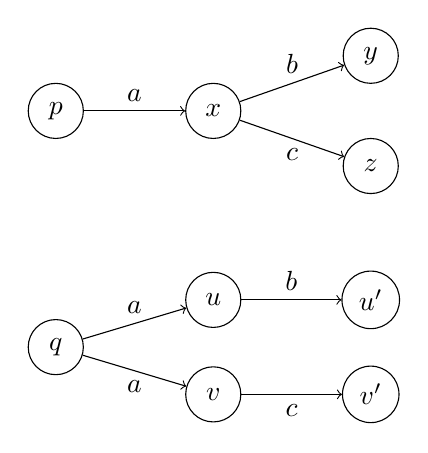
\begin{tikzpicture}[->,node distance=1.5cm]
  \tikzstyle{state}=[circle,draw,minimum size=7mm]
  \node[state] (p0) at (0,0) {$p$};
  \node[state] (p1) at (2,0) {$x$};
  \node[state] (p2) at (4,0.7) {$y$};
  \node[state] (p3) at (4,-0.7) {$z$};
  \draw (p0) -- node[above] {$a$} (p1);
  \draw (p1) -- node[above] {$b$} (p2);
  \draw (p1) -- node[below] {$c$} (p3);

  \node[state] (q0) at (0,-3) {$q$};
  \node[state] (q1) at (2,-2.4) {$u$};
  \node[state] (q2) at (2,-3.6) {$v$};
  \node[state] (q3) at (4,-2.4) {$u'$};
  \node[state] (q4) at (4,-3.6) {$v'$};
  \draw (q0) -- node[above] {$a$} (q1);
  \draw (q0) -- node[below] {$a$} (q2);
  \draw (q1) -- node[above] {$b$} (q3);
  \draw (q2) -- node[below] {$c$} (q4);
\end{tikzpicture}
\end{center}

Both states have traces \(ab\) and \(ac\). But after action \(a\), the first system still offers both \(b\) and \(c\), while the second has already resolved the choice.

\begin{block}{Conclusion}
For branching-time logics, trace equivalence is too coarse.
\end{block}
}
\end{frame}

\begin{frame}{What should CTL observe?}
\Margines{
\(\CTL\) and \(\CTL^*\) can speak about the tree of possible futures.

\begin{block}{Examples}
\begin{itemize}
  \item \(EX\varphi\): there exists a next state satisfying \(\varphi\).
  \item \(AX\varphi\): every next state satisfies \(\varphi\).
  \item \(AG\,EF\,brake\): from every reachable state, braking remains possible.
\end{itemize}
\end{block}

\begin{block}{Problem}
A language of complete traces does not remember which choices were available at intermediate states.
\end{block}
}
\end{frame}

\begin{frame}{Simulation: branching inclusion}
\Margines{
Let \(T=(S,\Sigma,\rightarrow)\) be an LTS.

\begin{block}{Definition}
A relation \(R\subseteq S\times S\) is a simulation if \((s,t)\in R\) implies that for every action \(a\in\Sigma\) and every transition
\[
  s\xrightarrow{a}s'
\]
there exists a transition
\[
  t\xrightarrow{a}t'
\]
such that \((s',t')\in R\).
\end{block}

We write \(s\preceq t\) if some simulation contains \((s,t)\). Then \(t\) can reproduce every step of \(s\).
}
\end{frame}

\begin{frame}{Simulation and language inclusion}
\Margines{
For finite words, let
\[
  \mathcal L(s)=\{w\in\Sigma^* : \exists t\ s\xrightarrow{w}t\}.
\]

\begin{lemma}
If \(s\preceq t\), then
\[
  \mathcal L(s)\subseteq\mathcal L(t).
\]
\end{lemma}

\begin{block}{Proof idea}
Induction on \(\len{w}\). The first step of \(s\) can be matched by \(t\), and the successors are again related.
\end{block}

\begin{block}{Interpretation}
Simulation is a branching-time analogue of language inclusion.
\end{block}
}
\end{frame}

\begin{frame}{Simulation as abstraction}
\Margines{
Suppose that the concrete system is simulated by the abstract system:
\[
  \impl \preceq \absys.
\]

\begin{block}{Meaning}
The abstraction may have more behaviours.
\end{block}

\begin{block}{Universal verification principle}
If a universal property is true in the abstraction, then it is true in the concrete system.
\end{block}

\begin{block}{Caution}
Simulation is not an equivalence. It is useful for refinement and for preservation of suitable logical fragments.
\end{block}
}
\end{frame}

\begin{frame}{Which CTL fragments are preserved by simulation?}
\Margines{
Use label-preserving simulation on Kripke structures: if \(s\preceq t\), then \(L(s)=L(t)\) and every successor of \(s\) is matched by a successor of \(t\).

\begin{theorem}
If \(s\preceq t\), then:
\begin{enumerate}
  \item for every positive existential CTL formula \(\varphi\),
  \[
    M,s\models\varphi \quad\Longrightarrow\quad M,t\models\varphi;
  \]
  \item for every positive universal CTL formula \(\varphi\),
  \[
    M,t\models\varphi \quad\Longrightarrow\quad M,s\models\varphi.
  \]
\end{enumerate}
\end{theorem}

\begin{block}{Positive}
Negation is allowed only in front of atomic propositions.
\end{block}
}
\end{frame}

\begin{frame}{Why full CTL needs equivalence}
\Margines{
Full \(\CTL\) and \(\CTL^*\) contain both existential and universal path quantification, and they are closed under negation.

\begin{block}{Consequence}
A one-way simulation is usually not enough to preserve all formulas.
\end{block}

\begin{center}
\Large
\[
\text{one-way matching}
\quad\leadsto\quad
\text{preservation of fragments}
\]
\[
\text{two-way matching}
\quad\leadsto\quad
\text{logical equivalence}
\]
\end{center}

\begin{block}{Next goal}
Define the two-way version: bisimulation.
\end{block}
}
\end{frame}

\begin{frame}{Bisimulation: branching equivalence}
\Margines{
\begin{block}{Definition}
A relation \(B\subseteq S\times S\) is a bisimulation if \((s,t)\in B\) implies that for every \(a\in\Sigma\):
\begin{enumerate}
  \item every transition \(s\xrightarrow{a}s'\) can be matched by some \(t\xrightarrow{a}t'\) with \((s',t')\in B\);
  \item every transition \(t\xrightarrow{a}t'\) can be matched by some \(s\xrightarrow{a}s'\) with \((s',t')\in B\).
\end{enumerate}
\end{block}

\begin{block}{Notation}
\[
  s\sim t
\]
means that \(s\) and \(t\) are contained in some bisimulation.
\end{block}
}
\end{frame}

\begin{frame}{The greatest bisimulation}
\Margines{
\begin{lemma}
The union of any family of bisimulations is again a bisimulation.
\end{lemma}

\begin{block}{Corollary}
There is a greatest bisimulation relation. It is called \emph{bisimilarity} and denoted by \(\sim\).
\end{block}

\begin{lemma}
Bisimilarity is an equivalence relation.
\end{lemma}

\begin{block}{Proof idea}
Reflexivity follows from the identity relation. Symmetry is built into the definition. Transitivity follows because the composition of two bisimulations is again a bisimulation.
\end{block}
}
\end{frame}

\begin{frame}{Bisimulation game}
\Margines{
A position is a pair of states \((s,t)\).

\begin{block}{One round}
\begin{enumerate}
  \item Spoiler chooses one side, for example \(s\), and a transition
  \[
    s\xrightarrow{a}s'.
  \]
  \item Duplicator must answer with a transition with the same label
  \[
    t\xrightarrow{a}t'.
  \]
  \item The next position is \((s',t')\).
\end{enumerate}
\end{block}

\begin{block}{Winning condition}
Duplicator wins infinite plays. Spoiler wins if Duplicator cannot match a move.
\end{block}
}
\end{frame}

\begin{frame}{Game characterisation}
\Margines{
\begin{theorem}
For states of an LTS,
\[
  s\sim t
\]
if and only if Duplicator has a winning strategy in the bisimulation game from \((s,t)\).
\end{theorem}

\begin{block}{Meaning}
Bisimilarity means that no finite interaction experiment can expose a difference between the two states.
\end{block}

\begin{block}{Connection with logic}
A winning strategy for Spoiler can be read as a finite distinguishing modal formula.
\end{block}
}
\end{frame}

\begin{frame}{What we prove about logic}
\Margines{

\begin{block}{HMS is a fragment of CTL}
  CTL restricted to AX, EX. 
\end{block}

\begin{block}{Two directions for finite Kripke structures}
\begin{enumerate}
  \item If \(s\sim t\), then they satisfy the same \(\CTL^*\) formulas.
  \item If \(s\not\sim t\), then some state-labelled \(\HML\) formula distinguishes them.
\end{enumerate}
\end{block}

\begin{block}{Theorem}
Bisimulation is exactly the equivalence induced by \(\HML\), \(\CTL\), and \(\CTL^*\) on finite systems.
\end{block}
}
\end{frame}

\begin{frame}{Bisimulation for Kripke structures}
\Margines{
For Kripke structures, states are labelled by atomic propositions.

\begin{block}{Definition}
A relation \(B\subseteq S\times S\) is a bisimulation if \((s,t)\in B\) implies:
\begin{enumerate}
  \item \(L(s)=L(t)\),
  \item every successor of \(s\) is matched by a successor of \(t\),
  \item every successor of \(t\) is matched by a successor of \(s\).
\end{enumerate}
\end{block}

\begin{block}{Observation}
The equality \(L(s)=L(t)\) ensures that atomic propositions cannot distinguish bisimilar states.
\end{block}
}
\end{frame}

\begin{frame}{Hennessy--Milner logic}
\Margines{
\begin{block}{Syntax}
\[
\varphi ::= \top \mid \neg\varphi \mid \varphi_1\land\varphi_2 \mid \langle a\rangle\varphi,
\qquad a\in\Sigma.
\]
\end{block}

\begin{block}{Semantics of the modal operator}
\[
  s\models\langle a\rangle\varphi
\]
iff there exists \(s'\) such that
\[
  s\xrightarrow{a}s'
  \quad\text{and}\quad
  s'\models\varphi.
\]
\end{block}

\begin{block}{Derived operator}
\[
  [a]\varphi\equiv\neg\langle a\rangle\neg\varphi.
\]
\end{block}
}
\end{frame}

\begin{frame}{HML can see branching}
\Margines{
In the earlier example, the first state satisfies
\[
  \langle a\rangle
  (\langle b\rangle\top\land\langle c\rangle\top),
\]
while the second state does not.

\begin{block}{Reading}
There exists an \(a\)-successor from which both \(b\) and \(c\) are possible.
\end{block}

\begin{block}{Key point}
This formula does not describe only complete traces. It describes the shape of the branching tree.
\end{block}
}
\end{frame}

\begin{frame}{HML invariance}
\Margines{
\begin{theorem}
If \(s\sim t\), then for every \(\HML\) formula \(\varphi\),
\[
  s\models\varphi \iff t\models\varphi.
\]
\end{theorem}

\begin{block}{Proof idea}
Structural induction on \(\varphi\). The Boolean cases are immediate. For \(\langle a\rangle\psi\), use the matching \(a\)-transition provided by bisimulation and then apply the induction hypothesis to the successors.
\end{block}
}
\end{frame}

\begin{frame}{Finite-depth bisimulation approximants}
\Margines{
\[
B_0=S\times S.
\]
For \(k\geq 0\), \((s,t)\in B_{k+1}\) iff \(L(s)=L(t)\), and every successor of either state has a matching successor of the other with endpoints in \(B_k\).

\begin{block}{What depth means}
If \((s,t)\notin B_k\), Spoiler can expose a difference within \(k\) rounds; an HML distinguishing formula can be built with modal depth at most \(k\).
\end{block}

\begin{block}{Finite systems}
The sequence decreases and stabilizes, and its stable relation is bisimilarity.
\end{block}
}
\end{frame}

% \begin{frame}{Word approximants: a longer game move}
% \Margines{
% Write \(s\xrightarrow{w}s'\) when a finite path from \(s\) to \(s'\) has state-label word \(w\). Define \(B^{\mathrm{word}}_0=S\times S\). At level \(k+1\), Spoiler may choose any finite path word \(w\) on either side; Duplicator must match the same word and reach an endpoint pair in \(B^{\mathrm{word}}_k\).

% \begin{block}{Why bundle a word?}
% A move can inspect a whole finite path prefix at once, rather than just one transition. This makes temporal observations along paths more visible in the game.
% \end{block}

% \begin{block}{Connection to \(\CTL^*\)}
% Bisimulation matches paths pointwise, so the two paths have the same label word at every finite prefix. Word moves are useful intuition; the invariance proof still proceeds by matching infinite paths and induction on formulas.
% \end{block}
% }
% \end{frame}

\begin{frame}{Hennessy--Milner theorem}
\Margines{
\begin{theorem}
For finite LTSs,
\[
  s\sim t
  \quad\Longleftrightarrow\quad
  \forall\varphi\in\HML:
  s\models\varphi \iff t\models\varphi.
\]
\end{theorem}

\begin{block}{Proof idea: \(\Rightarrow\)}
This is HML invariance.
\end{block}

\begin{block}{Proof idea: \(\Leftarrow\)}
If \(s\not\sim t\), then Spoiler wins the finite bisimulation game from \((s,t)\). The winning strategy can be translated into an HML formula that is true in one state and false in the other.
\end{block}
}
\end{frame}

\begin{frame}{CTL* invariance}
\Margines{
\begin{theorem}
If two states of a Kripke structure are bisimilar, then they satisfy the same \(\CTL^*\) state formulas.
\end{theorem}

\[
  s\sim t
  \quad\Longrightarrow\quad
  \forall\varphi\in\CTL^*:
  \big(M,s\models\varphi \iff M,t\models\varphi\big).
\]

\begin{block}{Proof idea}
A bisimulation matches every infinite path pointwise. Matched paths have identical label words, so structural induction gives the same truth value for every \(\CTL^*\) path formula, and hence every state formula.
\end{block}
}
\end{frame}



\begin{frame}{Hierarchy of abstractions}
\Margines{
\begin{center}
\Large
\[
  s\sim t
  \quad\Longrightarrow\quad
  s\equiv_{\mathrm{tr}}t
\]
\[
  s\preceq t
  \quad\Longrightarrow\quad
  \mathcal L(s)\subseteq\mathcal L(t)
\]
\end{center}

\begin{block}{But}
The converse implications fail in general. Trace language semantics forgets branching information.
\end{block}

\begin{block}{Moral}
The stronger the logic, the richer the abstraction needed to preserve it.
\end{block}
}
\end{frame}

\begin{frame}{The abstraction table}
\Margines{
\begin{center}
\small
\renewcommand{\arraystretch}{1.35}
\resizebox{\textwidth}{!}{%
\begin{tabular}{|c|c|c|}
\hline
Logic / view & inclusion / refinement & equivalence \\
\hline
\(\LTL\) & language inclusion & language equivalence \\
\hline
positive existential \(\CTL\) & simulation: concrete \(\Rightarrow\) abstract & not exact \\
\hline
positive universal \(\CTL\) & simulation: abstract \(\Rightarrow\) concrete & not exact \\
\hline
\(\HML,\ \CTL,\ \CTL^*\) & -- & bisimulation \\
\hline
\end{tabular}}
\end{center}

\begin{block}{Important caution}
For full \(\CTL\) and \(\CTL^*\), bisimulation is the robust equivalence. Simulation is a preorder useful for abstraction and for preservation of suitable fragments.
\end{block}
}
\end{frame}

\begin{frame}{Summary}
\Margines{
\begin{itemize}
  \item A logic determines what observations matter.
  \item \(\LTL\) observes trace languages, so language inclusion and equivalence are natural.
  \item \(\CTL\) and \(\CTL^*\) observe branching, so trace languages are not enough.
  \item Simulation is a branching analogue of inclusion and preserves suitable fragments.
  \item Bisimulation is the branching equivalence induced by \(\HML\), \(\CTL\), and \(\CTL^*\) on finite systems.
\end{itemize}
}
\end{frame}

\begin{frame}{Next step}
\Margines{
\begin{block}{Algorithmic question}
If bisimulation is the right abstraction for branching-time logics, can we compute it efficiently?
\end{block}

\begin{block}{Answer}
For finite systems, yes: by partition refinement.
\end{block}

\begin{block}{Next file}
We compute the coarsest partition stable under successor observations.
\end{block}
}
\end{frame}

\end{document}
